
\documentclass[border=10pt, 12pt]{standalone}
\usepackage[svgnames]{xcolor}
\usepackage{amsmath}
\usepackage{pgfplots}
\pgfplotsset{compat=newest}
\usepackage[sfdefault]{FiraSans}
\usepackage{FiraMono}
\renewcommand*\familydefault{\sfdefault}
\begin{document}
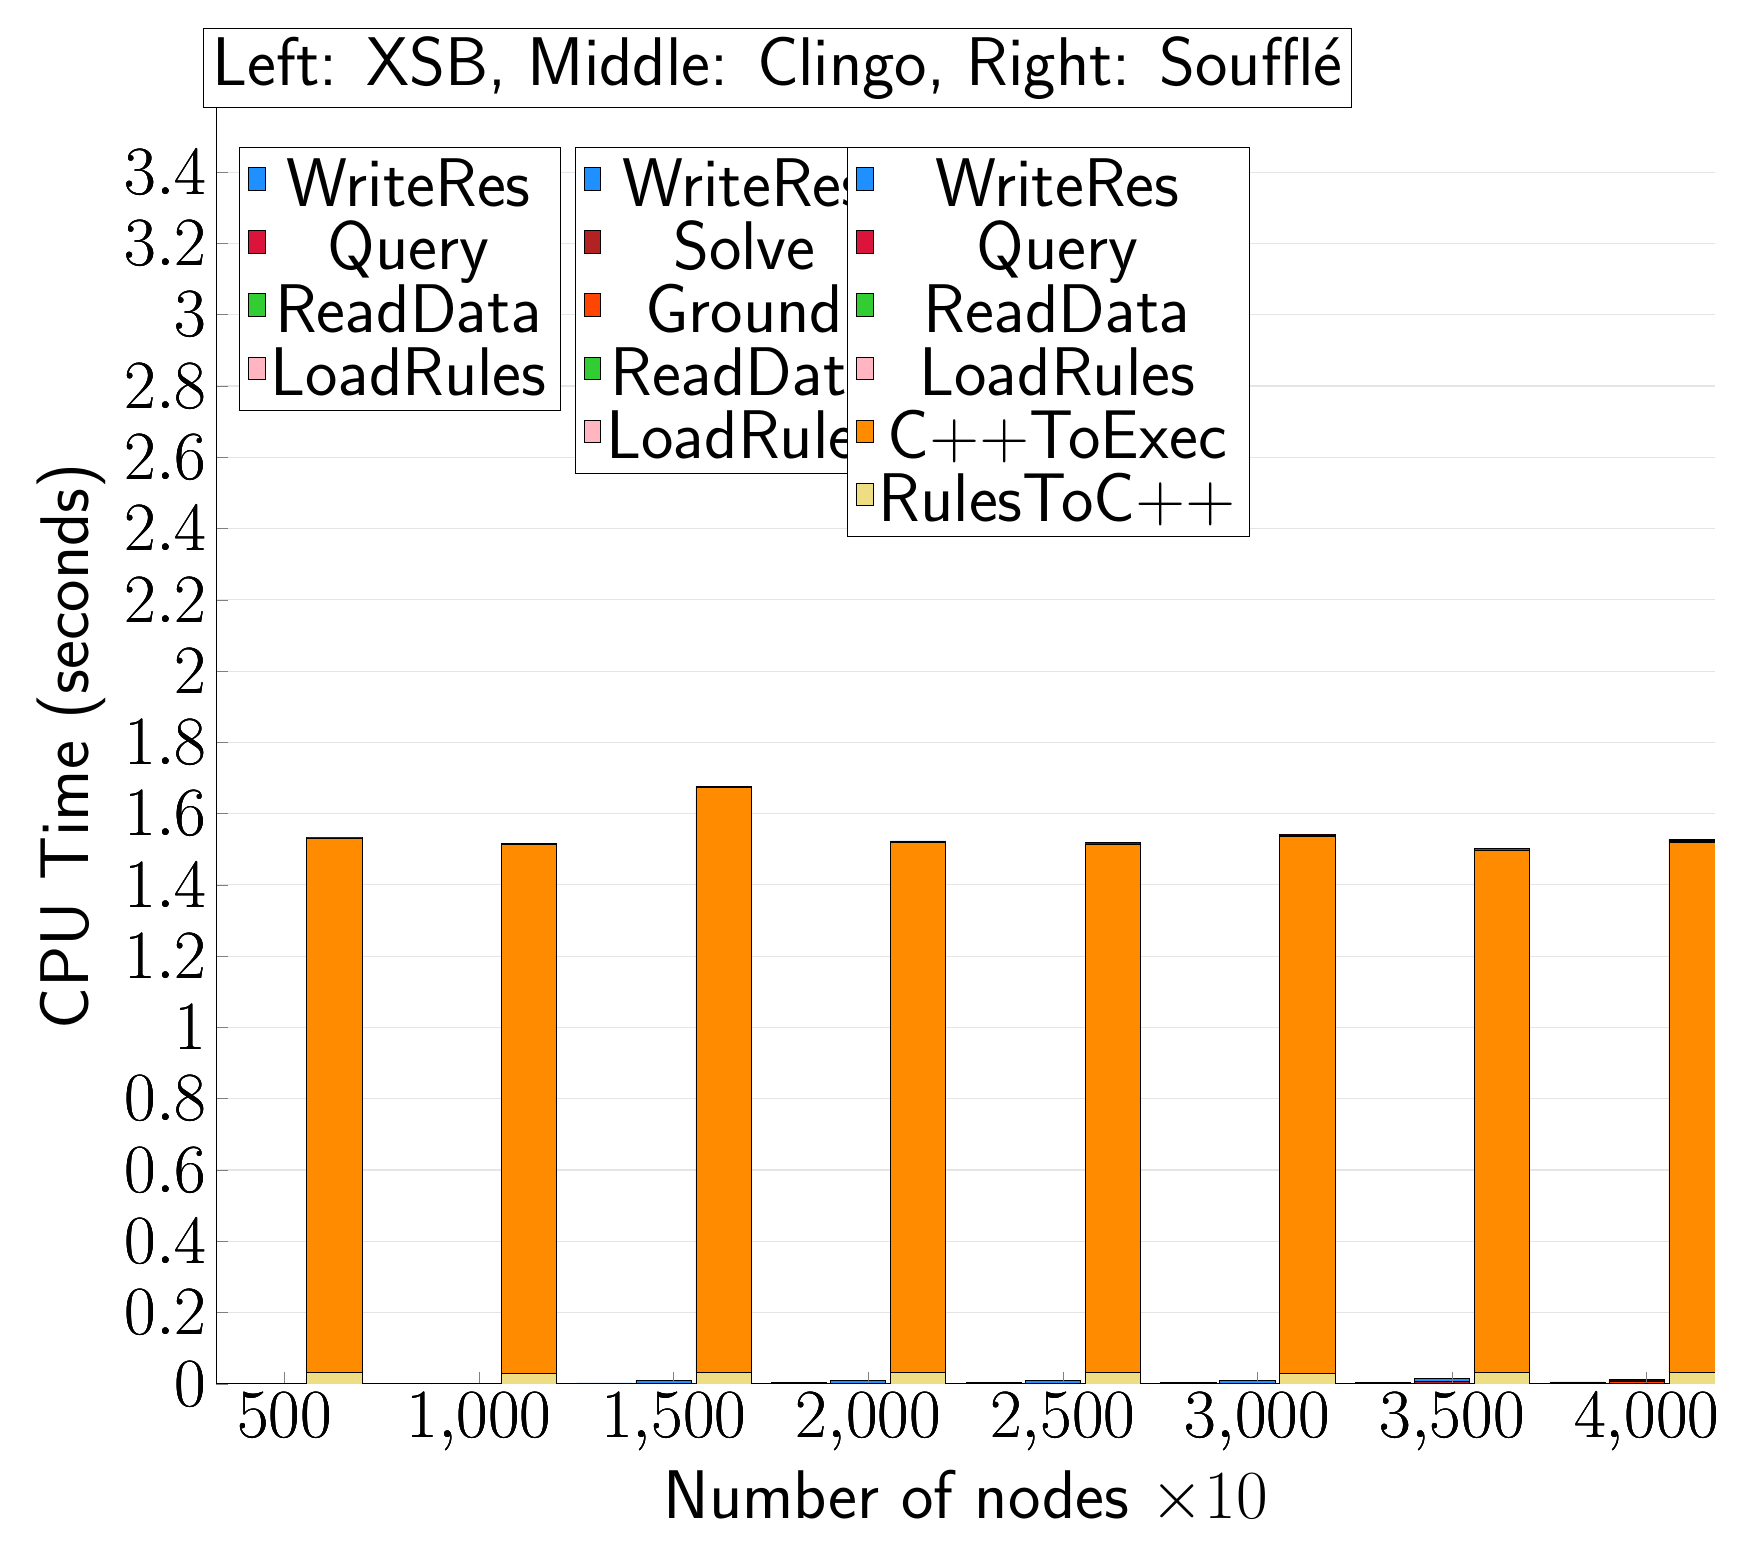
\begin{tikzpicture}
	\begin{axis}[bar shift=-25pt,
			ybar stacked,
			width=1.7\textwidth,
			bar width=0.7cm,
			ymajorgrids, tick align=inside,
			major grid style={draw=gray!20},
			xtick=data,
			ymin=0, ymax=3.579,
			axis x line*=bottom,
			axis y line*=left,
			enlarge x limits=0.05,
			legend style={
					at={(0.23, 0.97)},
					anchor=north east,
					legend columns=1,
					font=\Huge,
				},
			ylabel={CPU Time (seconds)},
			xlabel={Number of nodes $\times 10$},
			label style={font=\Huge},
			tick label style={font=\Huge},
		]
		\addlegendimage{fill=DodgerBlue, draw=black, line width=0.2pt}
		\addlegendentry{WriteRes}
		\addlegendimage{fill=Crimson, draw=black, line width=0.2pt}
		\addlegendentry{Query}
		\addlegendimage{fill=LimeGreen, draw=black, line width=0.2pt}
		\addlegendentry{ReadData}
		\addlegendimage{fill=LightPink, draw=black, line width=0.2pt}
		\addlegendentry{LoadRules}
		\addplot +[fill=LightPink, draw=black, line width=0.2pt] coordinates {
				(500, 0.0006129000000000001)
				(1000, 0.0006027999999999999)
				(1500, 0.0005951000000000001)
				(2000, 0.0006196999999999997)
				(2500, 0.0006086000000000002)
				(3000, 0.0006031999999999997)
				(3500, 0.0006123999999999997)
				(4000, 0.0006034999999999999)
			};
		\addplot +[fill=LimeGreen, draw=black, line width=0.2pt] coordinates {
				(500, 0.0001825999999999997)
				(1000, 0.0002252999999999998)
				(1500, 0.00027229999999999995)
				(2000, 0.0003208000000000003)
				(2500, 0.0003601)
				(3000, 0.0004059000000000004)
				(3500, 0.00046)
				(4000, 0.0004889999999999996)
			};
		\addplot +[fill=Crimson, draw=black, line width=0.2pt] coordinates {
				(500, 6.50000000000005e-05)
				(1000, 0.0001103000000000006)
				(1500, 0.00016129999999999988)
				(2000, 0.00021239999999999947)
				(2500, 0.0002552999999999999)
				(3000, 0.0003301000000000006)
				(3500, 0.00038219999999999997)
				(4000, 0.00043890000000000015)
			};
		\addplot +[fill=DodgerBlue, draw=black, line width=0.2pt] coordinates {
				(500, 0.0005599999999999995)
				(1000, 0.0010156999999999994)
				(1500, 0.0014642000000000001)
				(2000, 0.0018939000000000004)
				(2500, 0.0023398)
				(3000, 0.0027863999999999996)
				(3500, 0.0032530000000000002)
				(4000, 0.0037355)
			};
	\end{axis}

	\begin{axis}[bar shift=-3.7pt,
			ybar stacked,
			width=1.7\textwidth,
			bar width=0.7cm,
			ymajorgrids, tick align=inside,
			major grid style={draw=none},
			xtick=data,
			ymin=0, ymax=3.579,
			axis x line*=none,
			axis y line*=none,
			enlarge x limits=0.05,
			legend style={
					at={(0.454, 0.97)},
					anchor=north east,
					legend columns=1,
					font=\Huge,
				},
			label style={font=\Huge},
			tick label style={font=\Huge},
		]
		\addlegendimage{fill=DodgerBlue, draw=black, line width=0.2pt}
		\addlegendentry{WriteRes}
		\addlegendimage{fill=FireBrick, draw=black, line width=0.2pt}
		\addlegendentry{Solve}
		\addlegendimage{fill=OrangeRed, draw=black, line width=0.2pt}
		\addlegendentry{Ground}
		\addlegendimage{fill=LimeGreen, draw=black, line width=0.2pt}
		\addlegendentry{ReadData}
		\addlegendimage{fill=LightPink, draw=black, line width=0.2pt}
		\addlegendentry{LoadRules}
		\addplot +[fill=LightPink, draw=black, line width=0.2pt] coordinates {
				(500, 0.0)
				(1000, 0.0)
				(1500, 0.0)
				(2000, 0.0)
				(2500, 0.0)
				(3000, 0.0)
				(3500, 0.0)
				(4000, 0.0)
			};
		\addplot +[fill=LimeGreen, draw=black, line width=0.2pt] coordinates {
				(500, 0.0)
				(1000, 0.0)
				(1500, 0.0)
				(2000, 0.0)
				(2500, 0.0)
				(3000, 0.0)
				(3500, 0.0)
				(4000, 0.0)
			};
		\addplot +[fill=OrangeRed, draw=black, line width=0.2pt] coordinates {
				(500, 0.0)
				(1000, 0.0)
				(1500, 0.0)
				(2000, 0.0009999999999999998)
				(2500, 0.0)
				(3000, 0.0)
				(3500, 0.0019999999999999996)
				(4000, 0.007999999999999997)
			};
		\addplot +[fill=FireBrick, draw=black, line width=0.2pt] coordinates {
				(500, 0.0)
				(1000, 0.0)
				(1500, 0.0)
				(2000, 0.0)
				(2500, 0.0)
				(3000, 0.0)
				(3500, 0.004999999999999999)
				(4000, 0.0019999999999999996)
			};
		\addplot +[fill=DodgerBlue, draw=black, line width=0.2pt] coordinates {
				(500, 0.0)
				(1000, 0.0)
				(1500, 0.009999999999999997)
				(2000, 0.008999999999999998)
				(2500, 0.009999999999999997)
				(3000, 0.009999999999999997)
				(3500, 0.007999999999999997)
				(4000, 0.0019999999999999996)
			};
	\end{axis}

	\begin{axis}[bar shift=18pt,
			ybar stacked,
			width=1.7\textwidth,
			bar width=0.7cm,
			ymajorgrids, tick align=inside,
			major grid style={draw=none},
			xtick=data,
			ymin=0, ymax=3.579,
			axis x line*=none,
			axis y line*=none,
			enlarge x limits=0.05,
			legend style={
					at={(0.69, 0.97)},
					anchor=north east,
					legend columns=1,
					font=\Huge,
				},
			label style={font=\Huge},
			tick label style={font=\Huge},
		]
		\addlegendimage{fill=DodgerBlue, draw=black, line width=0.2pt}
		\addlegendentry{WriteRes}
		\addlegendimage{fill=Crimson, draw=black, line width=0.2pt}
		\addlegendentry{Query}
		\addlegendimage{fill=LimeGreen, draw=black, line width=0.2pt}
		\addlegendentry{ReadData}
		\addlegendimage{fill=LightPink, draw=black, line width=0.2pt}
		\addlegendentry{LoadRules}
		\addlegendimage{fill=DarkOrange, draw=black, line width=0.2pt}
		\addlegendentry{C++ToExec}
		\addlegendimage{fill=LightGoldenrod, draw=black, line width=0.2pt}
		\addlegendentry{RulesToC++}
		\addplot +[fill=LightGoldenrod, draw=black, line width=0.2pt] coordinates {
				(500, 0.031000000000000007)
				(1000, 0.030000000000000006)
				(1500, 0.031000000000000007)
				(2000, 0.031000000000000007)
				(2500, 0.031000000000000007)
				(3000, 0.030000000000000006)
				(3500, 0.031000000000000007)
				(4000, 0.031999999999999994)
			};
		\addplot +[fill=DarkOrange, draw=black, line width=0.2pt] coordinates {
				(500, 1.501)
				(1000, 1.483)
				(1500, 1.6430000000000002)
				(2000, 1.4880000000000002)
				(2500, 1.4840000000000002)
				(3000, 1.5059999999999998)
				(3500, 1.465)
				(4000, 1.4880000000000002)
			};
		\addplot +[fill=LightPink, draw=black, line width=0.2pt] coordinates {
				(500, 0.00010320000000000001)
				(1000, 0.00010799999999999998)
				(1500, 0.0)
				(2000, 0.00012440000000000004)
				(2500, 9.87e-05)
				(3000, 0.0001093)
				(3500, 0.0001248)
				(4000, 6.15e-05)
			};
		\addplot +[fill=LimeGreen, draw=black, line width=0.2pt] coordinates {
				(500, 0.00034520000000000004)
				(1000, 0.0004666999999999999)
				(1500, 0.00039789999999999997)
				(2000, 0.0007125)
				(2500, 0.0007843000000000001)
				(3000, 0.0008927000000000001)
				(3500, 0.0010725)
				(4000, 0.0010450999999999998)
			};
		\addplot +[fill=Crimson, draw=black, line width=0.2pt] coordinates {
				(500, 0.0006115)
				(1000, 0.0012253)
				(1500, 0.0011457)
				(2000, 0.002521)
				(2500, 0.0029353)
				(3000, 0.0035470999999999996)
				(3500, 0.0044519)
				(4000, 0.0045708)
			};
		\addplot +[fill=DodgerBlue, draw=black, line width=0.2pt] coordinates {
				(500, 0.0004273000000000001)
				(1000, 0.0006885)
				(1500, 0.000662)
				(2000, 0.0012106000000000003)
				(2500, 0.0012556)
				(3000, 0.001518)
				(3500, 0.0018306000000000004)
				(4000, 0.0018499999999999999)
			};
	\end{axis}


	\node[anchor=south, draw, fill=white] at (rel axis cs:0.42,1) {\Huge Left: XSB, Middle: Clingo, Right: Soufflé};
\end{tikzpicture}
\end{document}
